\section{Opis rezultata}
Mreža se s vremenom ponašala iznimno zanimljivo.
Već u prvih par koraka vrijednost ukupne funkcije gubitka ~\ref{eq:lokKlasLoss} brzo se spustila sa $\geq 50$ na $\leq 10$.
No nevjerojatno dugo joj je trebalo da se spusti na vrijednost $\leq 4$.
Razlog tome je pretpostavljam određeni broj \emph{false positive}-a (Slika ~\ref{fig:FalsePositive}) unutar skupa podataka.
Naime, \emph{false positive} slike nastale su primjenom transformacija nasumično generiranim parametrima koji su se našli na rubu prihvatljivih vrijednosti.
Nažalost, zbog velikog broja slika (nakon svih generiranja, pokušaja i treniranja $\geq 20000$) nisam ručno mogao izbaciti sve.
Ipak, smatram da je određeni mali broj takvih slika neophodan za uspješno treniranje slike. \\
Nakon ukupno $500 000$ koraka, tj. $80$ epoha po formuli ~\ref{eq:stepEpoch},  ukupni gubitak iznosio je $3.879$ gdje je po izgledu dosegao asimptotu.
\section{Prikaz rezultata}
Na slici ~\ref{fig:IndividualDigit} prikazana je prva uspješno detektirana i klasificirana slika, dotad ne viđena mreži.
Postotak pouzdanosti ($0.54$) je jasno na donjoj granici i naslućuje prve uspjehe prilagođenoj neuronskoj mreži koja nikad prije nije bila osmišljena za detekciju teksta.
\begin{figure}
	\subfloat[\emph{False positive} slika koja sadrži neodređeni element naizgled nevidljiv zbog nepravilnih transformacija primjenjenih na istom] {%
		
\includegraphics[width=0.45\linewidth]{false_positive} %
		\label{fig:FalsePositive}
	}
	\qquad
	\subfloat[Prva detekcija računalno generirane  znamenke 3 na slici uz mali postotak pouzdanosti] {%
		
\includegraphics[width=0.45\linewidth]{three} %
		\label{fig:IndividualDigit}
	}
\end{figure} \\
S vremenom, mreža je postajala sve pouzdanija te je nakon $\approx 350000$ koraka prvi puta prepoznala cijeli izraz, odnosno sve članove istog.
Priložene slike (~\ref{fig:ExpressionA} i ~\ref{fig:ExpressionB}) također nikad prije nisu bile viđene od mreže i dobar su primjer jer se jasno vidi kako, iako su slike identične, nakon određenog dodatnog broja koraka mreža preciznije određuje granice individualnih simbola i puno pouzdanije prenosi koji su. \\
\begin{figure}
	\subfloat[Pouzdanost i preciznost nakon $350000$ koraka] {%
		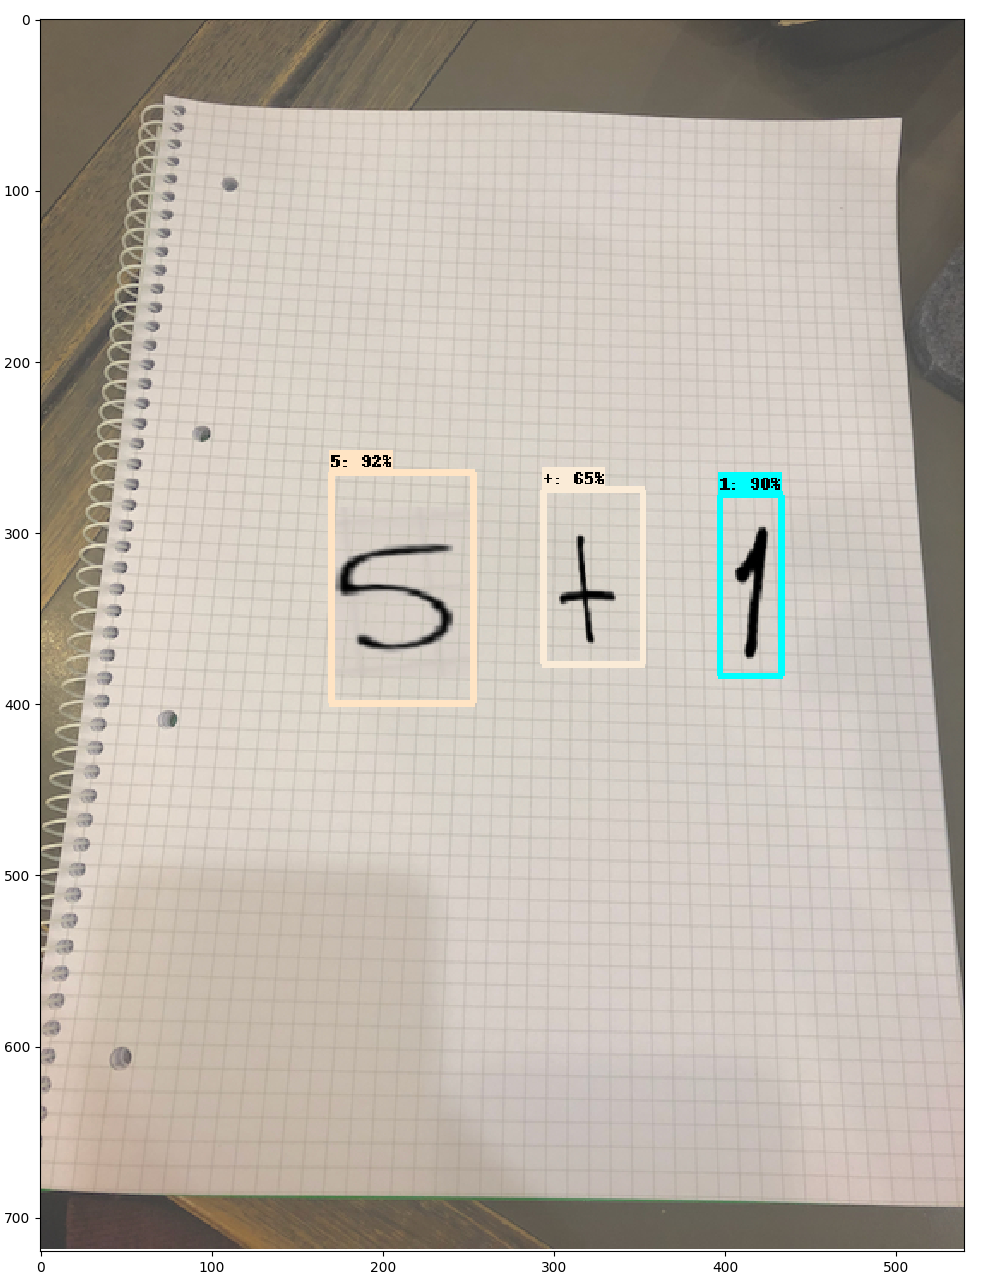
\includegraphics[width=0.45\linewidth]{first_generated_eqn} %
		\label{fig:ExpressionA}
	}
	\qquad
	\subfloat[Pouzdanost i preciznost nakon $500000$ koraka] {%
		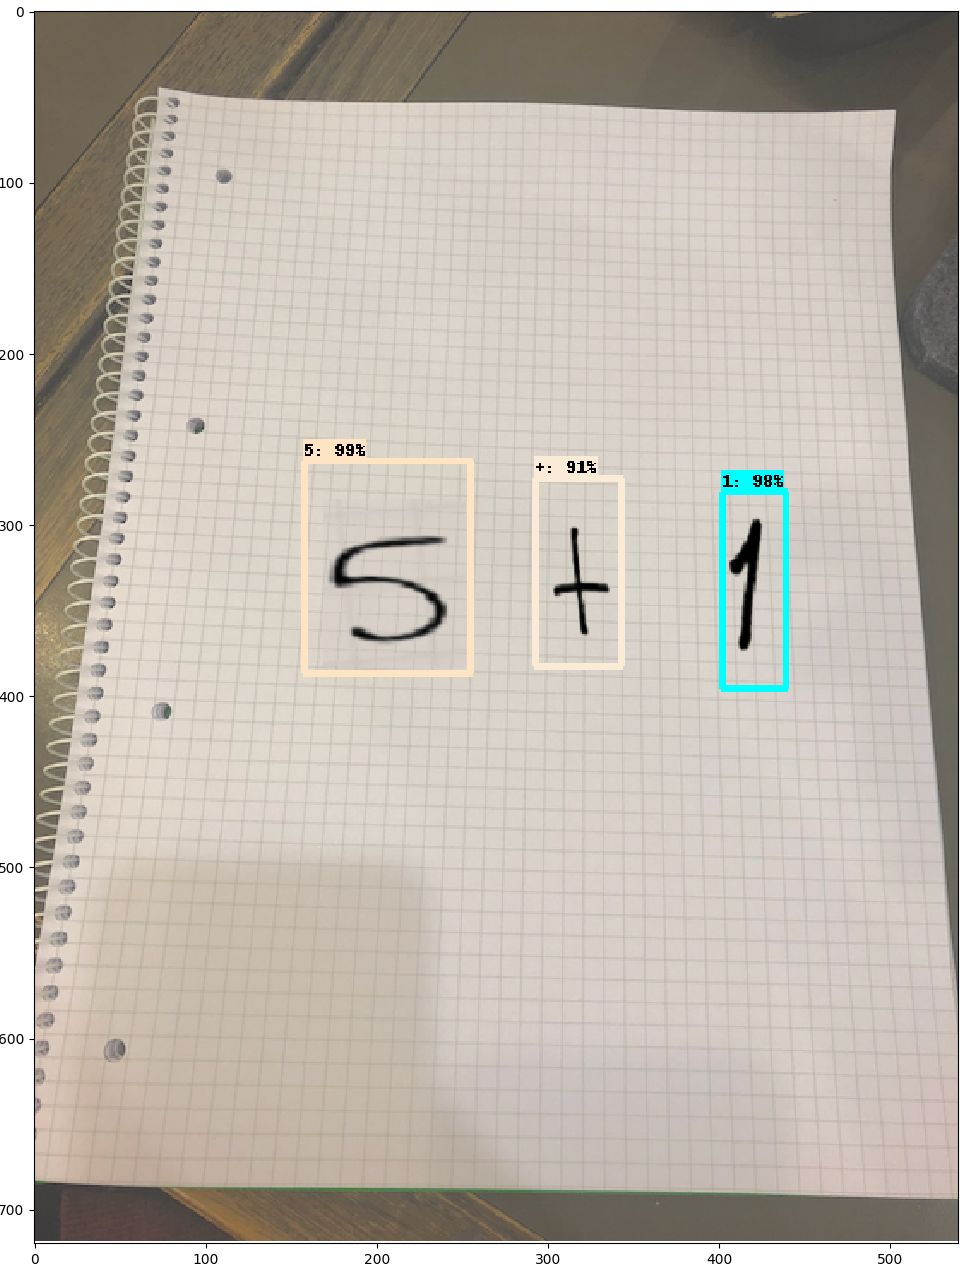
\includegraphics[width=0.45\linewidth]{last_generated_eqn} %
		\label{fig:ExpressionB}
	}
\end{figure} \\
Nakon završenog treninga bilo je zanimljivo probati je li mreža ušla u fazu \emph{prenaučenosti}-a što se vrlo lako moglo provjeriti dajući joj stvarni, rukom napisani primjer kojeg je bez problema detektirala i klasificirala (Slika ~\ref{fig:Handwritten}).
\begin{figure}[h!]
	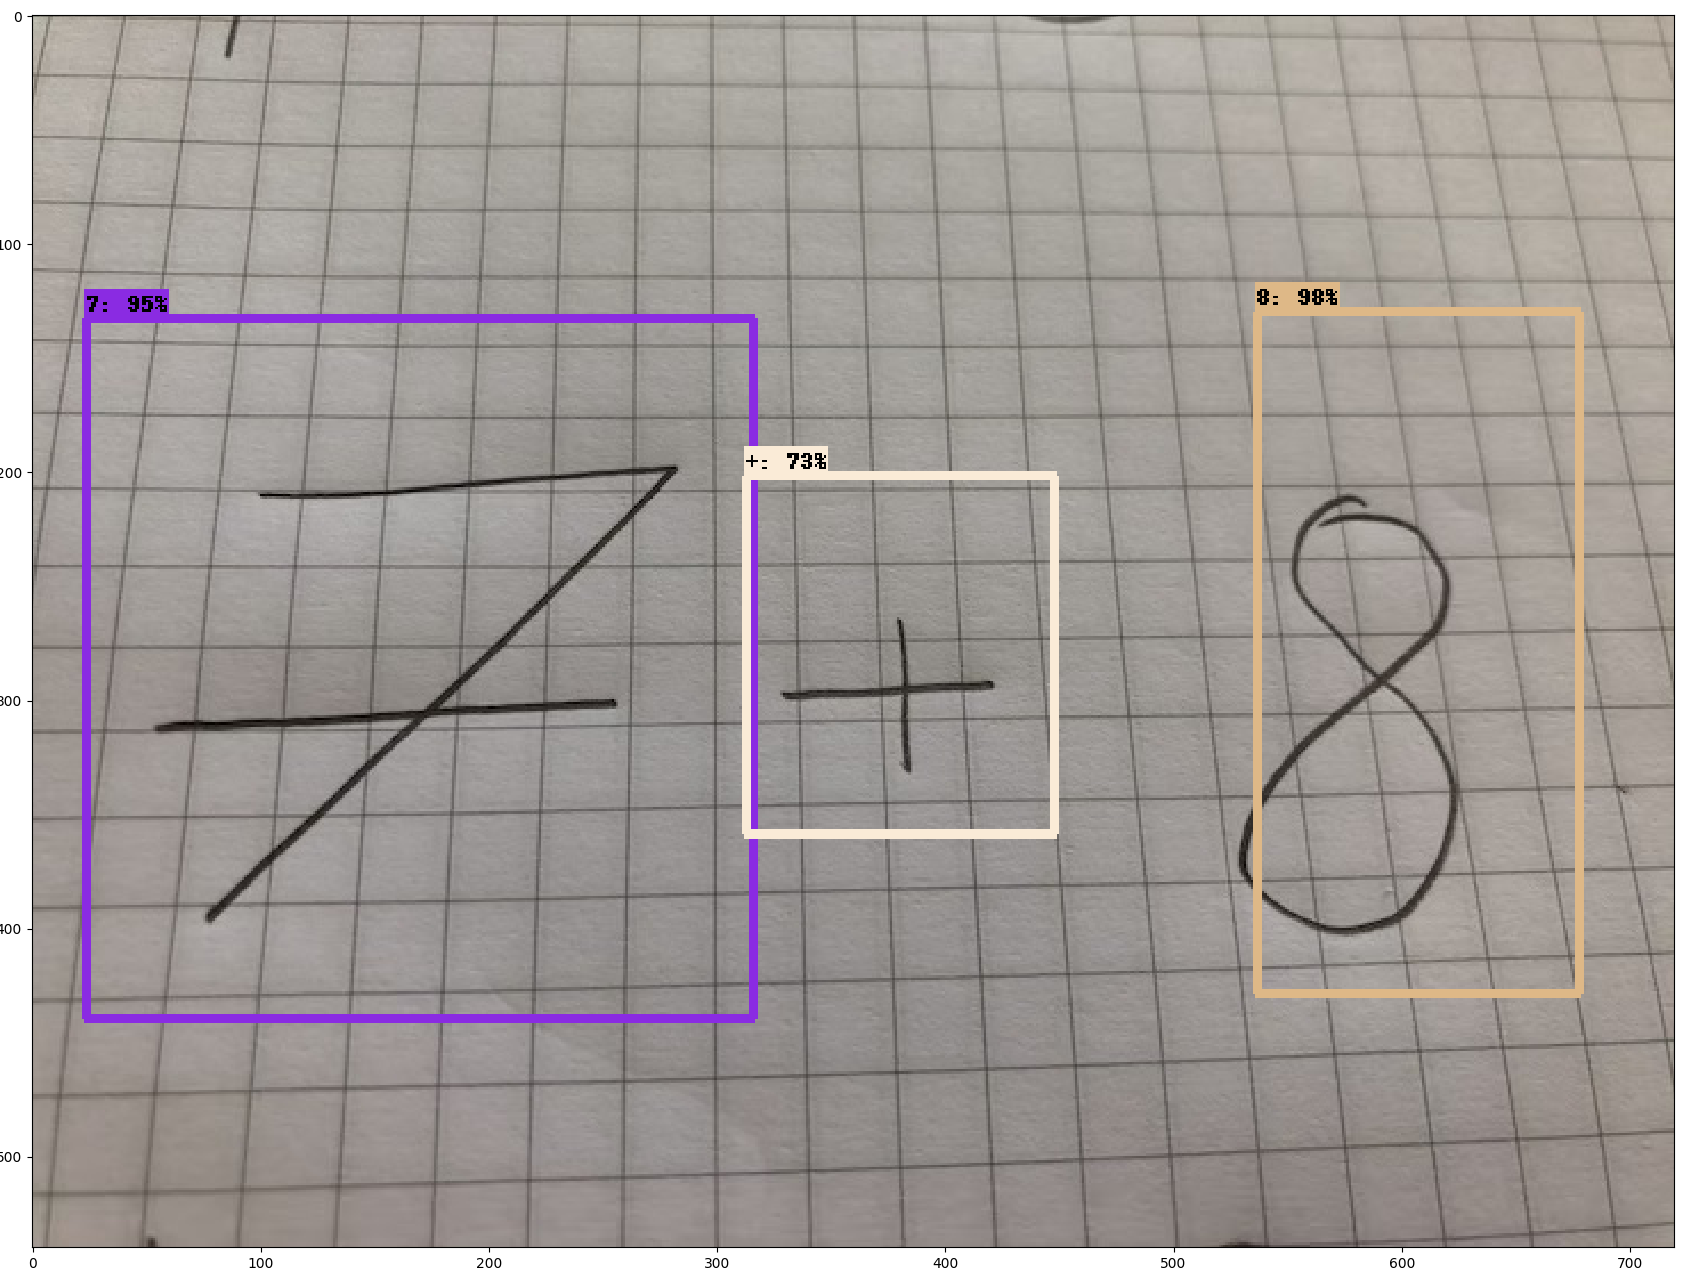
\includegraphics[width=0.5\linewidth]{handwritten}
	\caption{Jednostavan ručno napisan matematički izraz koji prikazuje uspjeh rada mreže na istom}
	\label{fig:Handwritten}
\end{figure}
\section{\emph{Tensorboard} rezultati}
Velika prednost korištenja \emph{Tensorflow}-a nad ostalim knjižnicama za duboko učenje je korištenje \emph{Tensorboard}-a koji fantastično i uživo prikazuje napredak učenja mreže zadanog zadatka.
Slika ~\ref{fig:losses} prikazuje način na koji \emph{Tensorboard} prikazuje gubitke kroz vrijeme, dok ~\ref{fig:totalLoss} prikazuje ukupan gubitak kroz vrijeme.
Naravno, naprednim korištenjem alata mogu se prikazati i ostale korisne stvari kao što je prikaz rada mreže na određenom broju slika uživo, no za moje potrebe, prikaz gubitka je bio dostatan za razumjevanje procesa učenja.
\begin{figure}
	\subfloat[Napredak dvije komponente gubitka kroz vrijeme] {%
		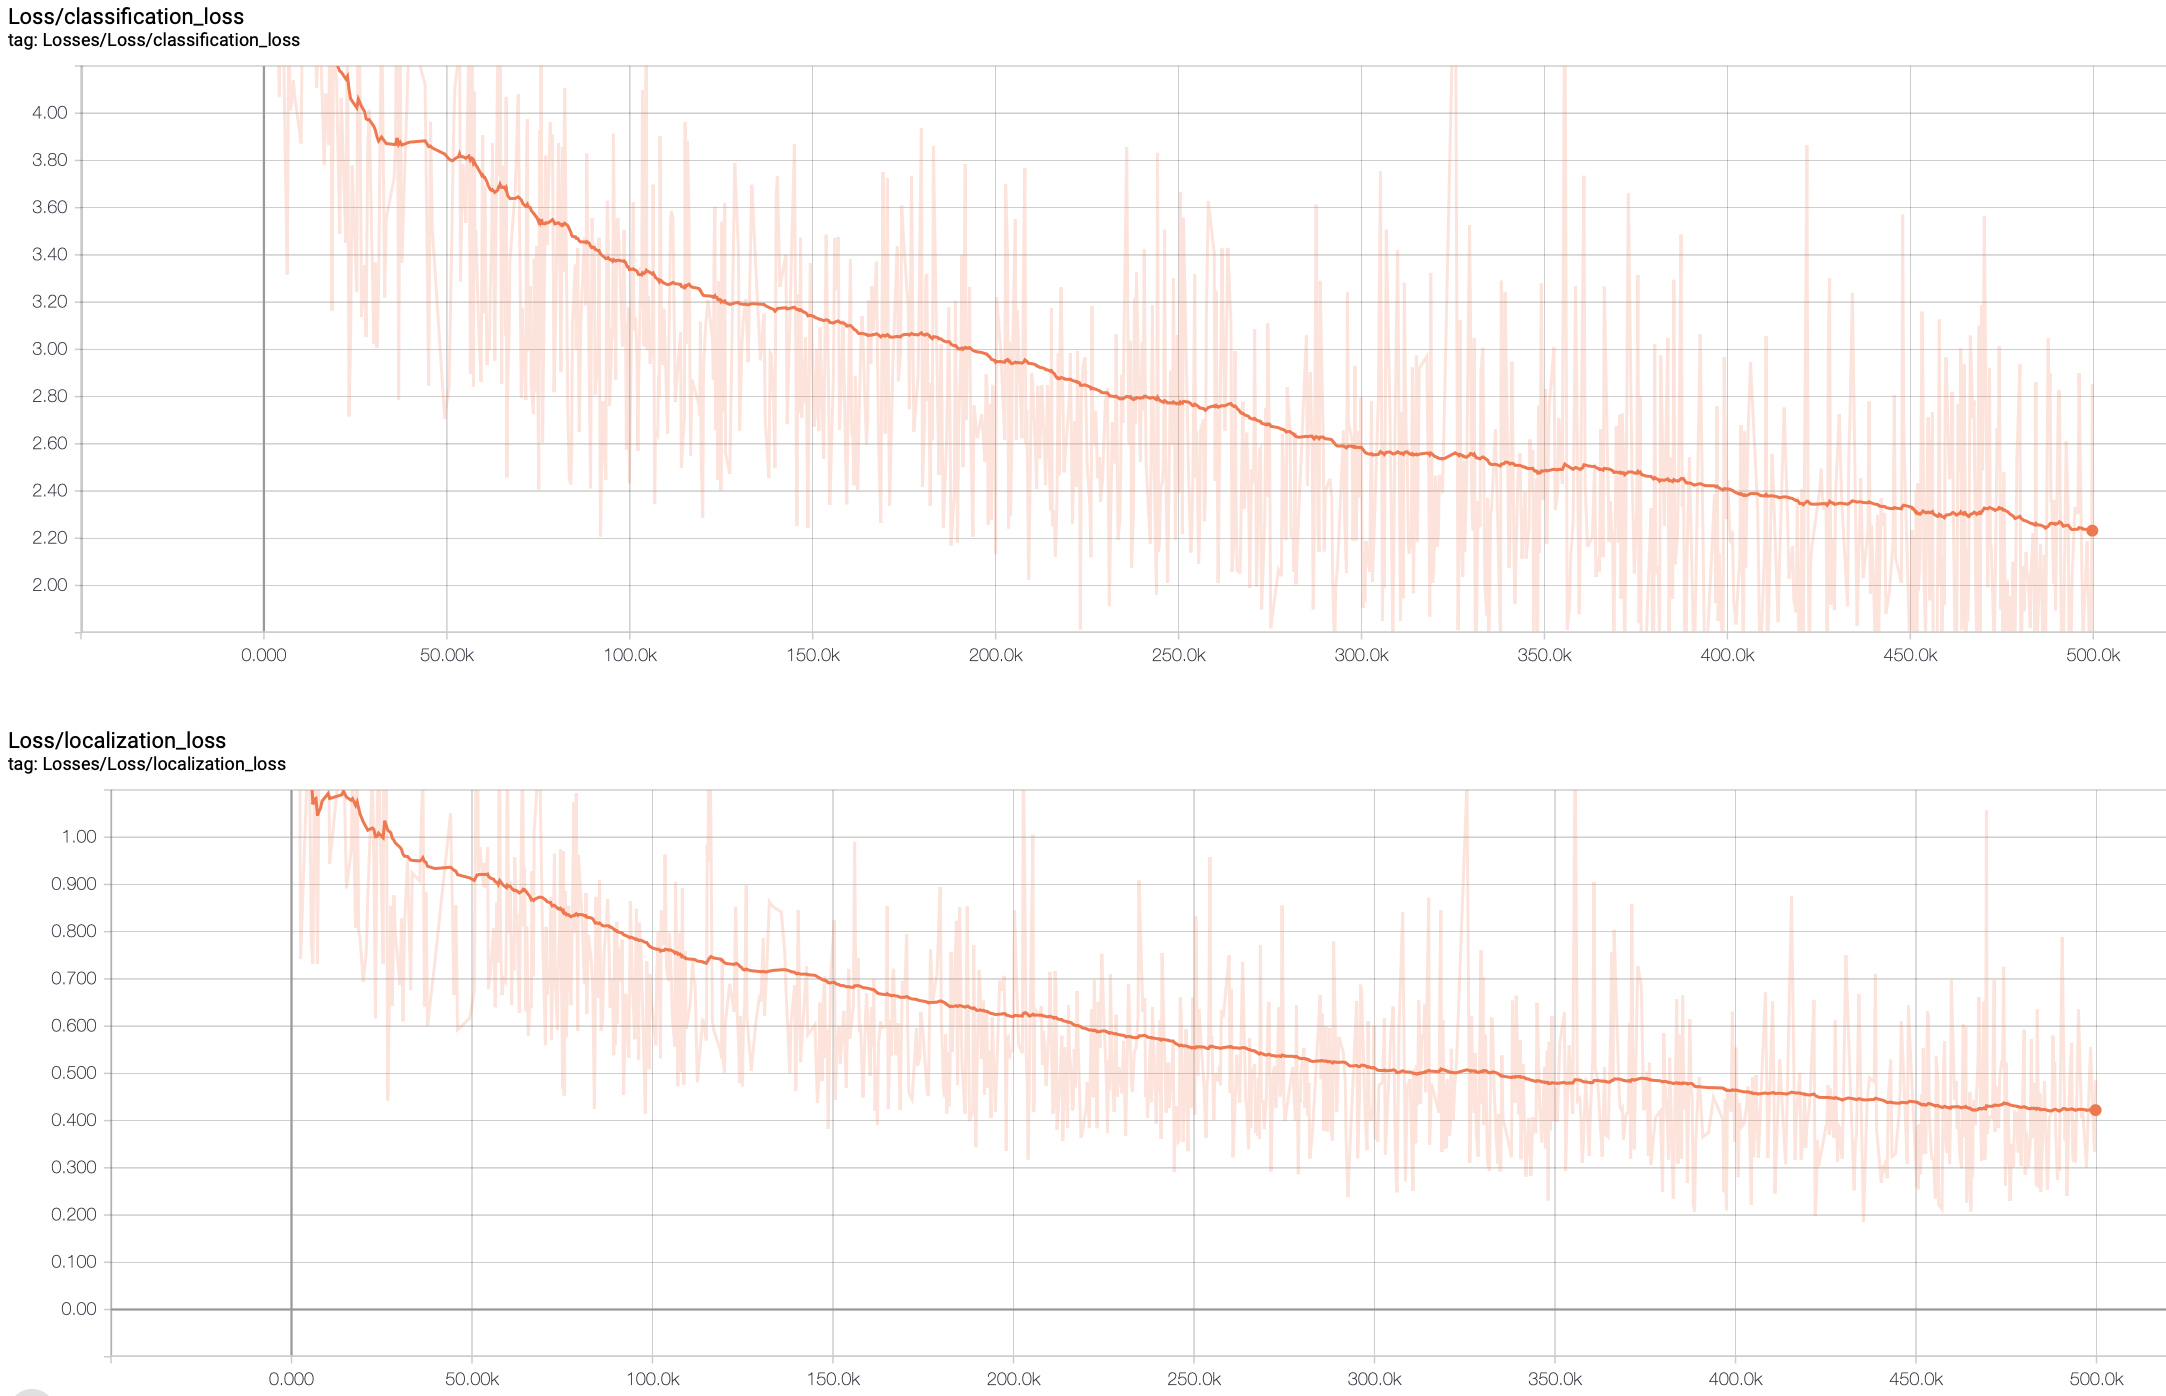
\includegraphics[width=1.0\linewidth]{losses} %
		\label{fig:losses}
	} \\
	\subfloat[Ukupan gubitak nastao od lokalizacijskog i klasifikacijskog gubitka kroz vrijeme] {%
		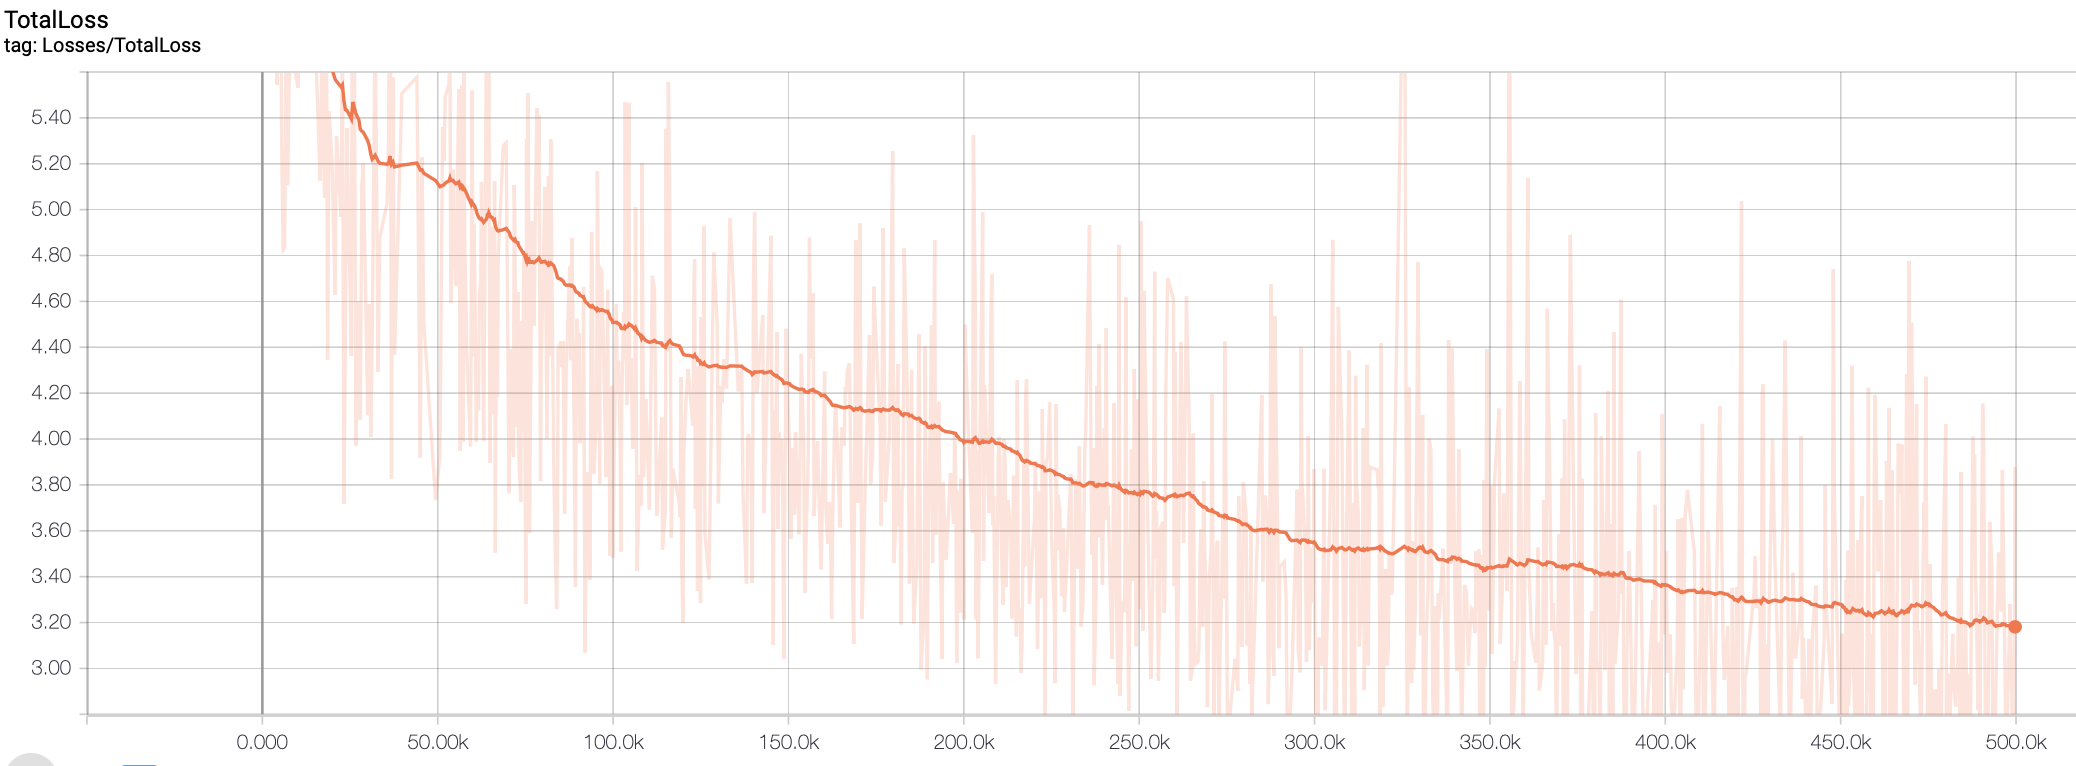
\includegraphics[width=1.0\linewidth]{total_loss} %
		\label{fig:totalLoss}
	}
\end{figure}
